\documentclass{exam}
\usepackage[utf8]{inputenc}
\usepackage{graphicx}
\begin{document}

\vspace{5mm}
\makebox[0.75\textwidth]{Full Name: Sajal Shrestha}

\vspace{5mm}
\makebox[0.75\textwidth]{CS622 ML Project-4}
\begin{questions}

\begin{figure}[htp]
    \centering
    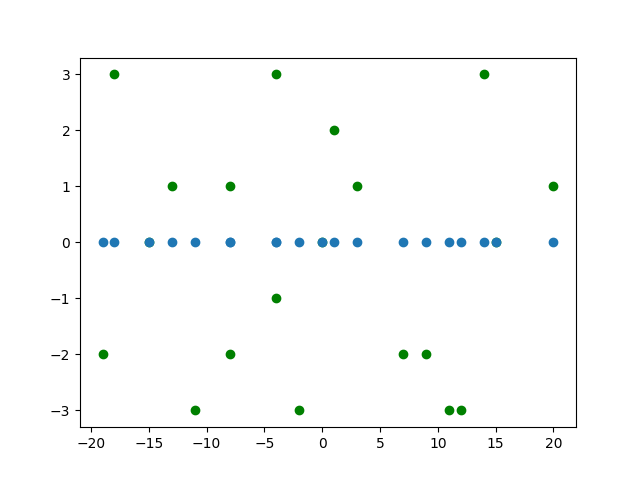
\includegraphics[width=17cm]{Figure_1.png}
    \caption{Original data Z as a scatter plot and the projected data Z\_star as a line.}
    \label{fig:plot}
\end{figure}
\vspace{\stretch{0.5}}

\question\textbf{Benefit to principal component analysis when dealing with higher dimensional feature vectors.}
\par\normalfont 
- Principal component analysis is a dimensionality-reduction method that is often used to reduce the dimensionality of large data sets.
We want to use more information in order to improve the accuracy of our model, as the dimensionality of the feature space increases, the number of configurations increases exponentially, and hence, the number of configurations covered by observation decreases.

\vspace{\stretch{0.5}}
\end{questions}
\clearpage
\end{document}